% !TEX root = ../main.tex
\subsubsection{Forward Detector}
\label{sssec::forward_detector}
    % The Forward Detector (FD) is an essential component of the CLAS12 spectrometer designed to detect particles scattered at small polar angles in the forward direction.
    % It consists of several subdetectors that play crucial roles in particle identification, tracking, and timing measurements.
    %
    % Based on its polar coverage, the FD can be divided into two: the Forward Tagger (FT) and the FD proper.
    % The former detects particles with a polar angle between $2.5\degree$ and $4.5\degree$.
    % The latter detects those with a polar angle between $5\degree$ and $35\degree$.
    % A detailed description of each subdetector systems is provided in the following paragraphs.
    %
    % The Forwards Micromegas Tracker (FMT) is part of the FD, but is not included in this list.
    % The detectors is explored in detail in Section \ref{ssec::forwardsmicromegastracker}.

    % !TEX root = ../main.tex
\paragraph{High Threshold Cherenkov Counter (HTCC)}
    \begin{wrapfigure}{l}{0.50\textwidth}
        \centering\frame{
        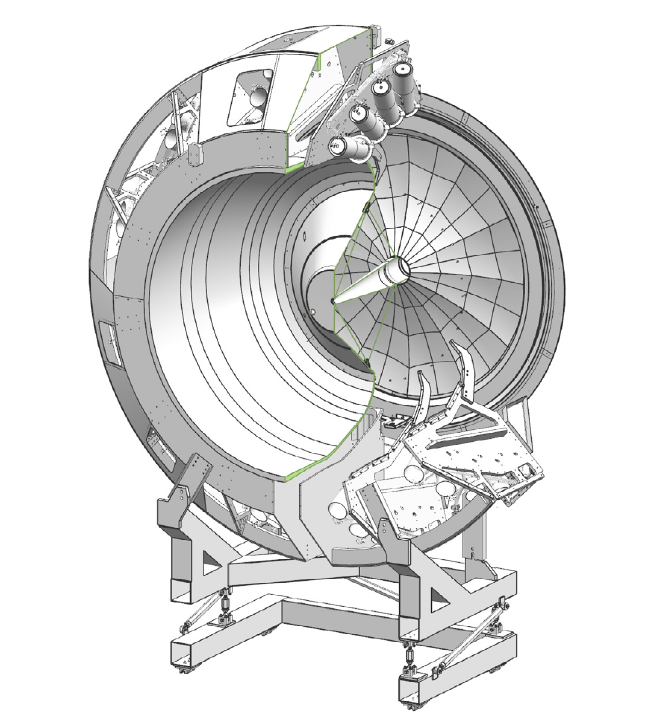
\includegraphics[width=\linewidth]{211htcc.png}}
        \caption[HTCC]{Render of the High Threshold Cherenkov Counter.
        The container spans a diameter of about 4.5 m. The mirror is seen at the downstream end to the right.
        The PMTs are mounted in 12 sectors and in groups of 4 at the outer perimeter of the container.
        Light collection uses additional Winston cones and 5-in PMTs with quartz windows.
        Source: \hyperlink{jlab.org/physics/hall-b/clas12}{CLAS12 wiki}.}
        \label{fig::htcc}
    \end{wrapfigure}

    The HTCC is specifically designed to separate electrons and positrons with momenta below 4.9 GeV from other charged particles.
    It achieves this through its capability for electron/positron identification, which provides high rejection of charged pions and low background noise.
    This is crucial for reliably identifying scattered electrons in an environment with a dense electromagnetic background.

    The HTCC is positioned downstream of the target and is fitted in between magnets, upstream of the forward tracking detectors.
    It ensures full azimuthal coverage, meaning it can detect particles emitted from any direction around its circumference.
    In terms of the polar angle, it spans from $5\degree$ to $35\degree$, covering a specific range of particle emission angles.
    Importantly, it has no blind areas in its complete solid angle coverage, meaning there are no regions where particles cannot be detected.

    Operating in dry CO2 gas at 1 atm pressure, the HTCC consists of a multi-focal mirror composed of 48 elliptical mirror facets.
    This mirror design enables the focusing of Cherenkov light produced by charged particles passing through the detector.
    The focused light is then detected by 48 Photomultiplier Tubes (PMTs), with each PMT featuring a quartz window of 125 mm in diameter.

    The PMTs are positioned within a magnetic field of up to $3.5\cdot 10^{-3}$ T, which is oriented along the axes of the phototubes.
    To minimize the impact of the magnetic field on the PMTs, they are surrounded along their lengths by a multi-layer magnetic shield.
    This shield includes active compensation coils, which further help in shielding the PMTs from the effects of the magnetic field.

    To minimize the effects of multiple scattering and its impact on the momentum analysis of charged tracks in the torus field, the HTCC mirror system is constructed using a backing structure made of low-density composite material.
    This choice of material helps to reduce the scattering of particles passing through the HTCC, thereby improving the accuracy of momentum measurements.

    Since the HTCC is located in front of the momentum analyzing torus magnet, it is important to minimize the presence of materials in the path of charged particles, except for the radiator gas.
    This is done to prevent interactions and disturbances that could affect the accuracy of momentum analysis.
    The HTCC is designed with this consideration in mind.

    In the HTCC, the density of solid material encountered by charged particles passing through its volume is approximately $135~\text{mg/cm}^2$.
    This low-density configuration ensures that the material contribution to multiple scattering is minimised, allowing for more precise momentum measurements of charged tracks.

    The HTCC also serves the purpose of generating a fast signal that can be used as a trigger for scattered electrons.
    This signal is utilised to identify and select scattered electrons for further analysis.

    In conjunction with the energy deposited in the electromagnetic calorimeters, the HTCC plays a role in the identification of electrons with specific energies.
    By combining the information from the HTCC and the electromagnetic calorimeters, the experiment can accurately identify electrons of interest based on their energy deposition patterns.

    A visual representation of the HTCC can be seen in Figure \ref{fig::htcc}, which provides a cut view of the detector and its components.

    Overall, the HTCC plays a crucial role in electron/positron identification by using a multi-focal mirror, PMTs, and a magnetic field setup.
    These components work together to ensure efficient detection and separation of electrons and positrons from other charged particles in a high-energy physics experiment environment.

    % !TEX root = ../main.tex
\paragraph{Drift Chambers (DC)}
    The forward tracking system in the experiment consists of three independent drift chambers in each of the six sectors of the torus magnet.
    These drift chambers serve as the primary tracking detectors and are supported by the six coils of the torus magnet.

    Each sector of the torus magnet contains a total of 36 layers in the drift chambers, with each layer having 112 sense wires.
    The sense wires are arranged in three regions, with each region comprising twelve layers.
    This configuration results in a total of 112 x 36 sense wires per sector.

    \begin{wrapfigure}{r}{0.50\textwidth}
        \frame{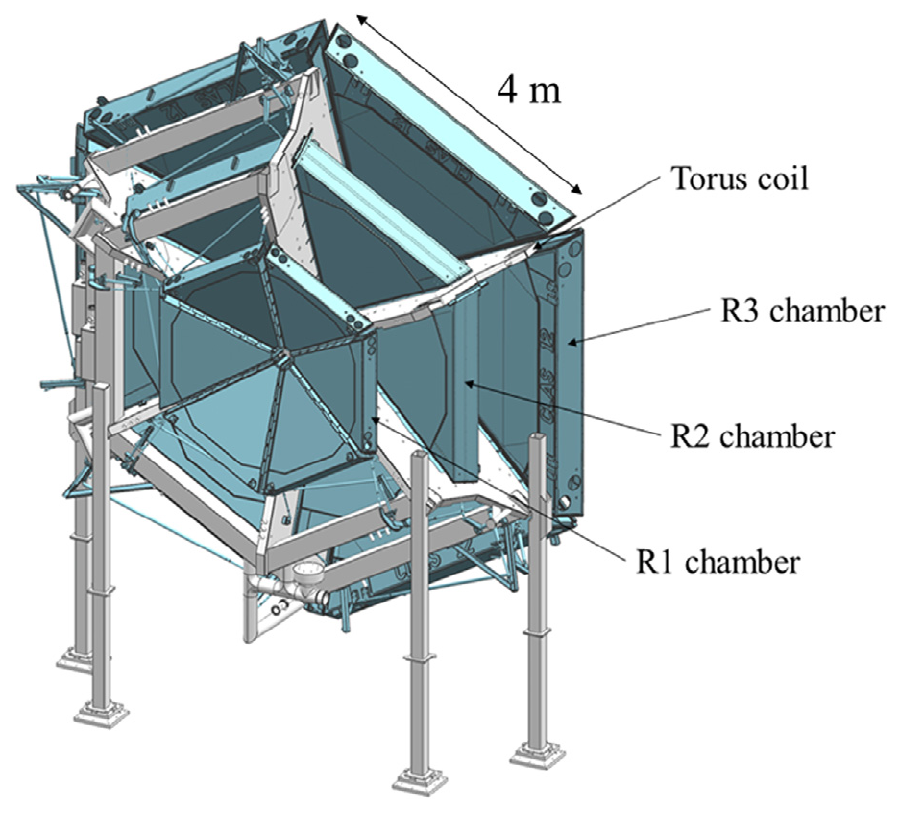
\includegraphics[width=\linewidth]{212dc.png}}
        \caption[DC]
        {Drift Chambers (DC) render.
        Each of the DC regions are denoted as R1, R2, and R3 in the figure.}
        \floatfoot{Source: \href{https://jlab.org/physics/hall-b/clas12}{CLAS12 wiki}.}
        \label{fig::11.212::dc}
    \end{wrapfigure}

    The arrangement of the drift chambers around the torus coil can be visualised in Figure \ref{fig::11.212::dc}.
    The figure shows the positioning of the three regions of the drift chambers in each sector of the torus magnet.

    In terms of location, the first region of the drift chambers is situated at the entrance to the torus magnetic field region.
    The second region is positioned inside the magnet, where the magnetic field is close to its maximum strength.
    Finally, the third region is located downstream of the torus magnet, in a low magnetic field space.

    This arrangement of the drift chambers around the torus magnet provides independent and redundant tracking capabilities in each of the six torus sectors.
    It allows for precise reconstruction of charged particle trajectories and momentum measurements in the experiment.

    Each of the three regions in the drift chambers consists of six "superlayers," where each superlayer comprises two layers.
    The wires in one layer are strung at a stereo angle of $+6\degree$ relative to the sector midplane, while the wires in the other layer are strung at a stereo angle of $-6\degree$.
    This stereo configuration provides excellent resolution in the polar angle ($\Delta\theta < 2 ~\text{mrad}$) and good resolution in the azimuthal scattering angle ($\Delta\phi < 2 ~\text{mrad}$).

    \begin{wrapfigure}{l}{0.50\textwidth}
        \frame{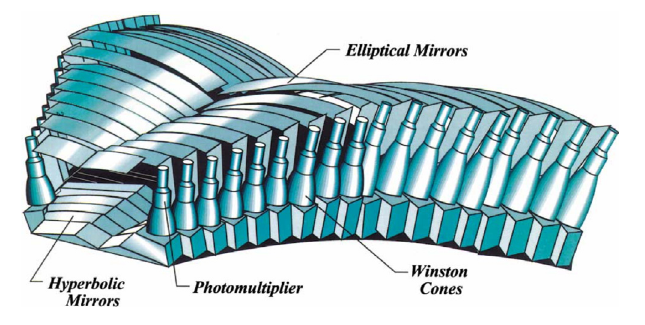
\includegraphics[width=\linewidth]{213ltcc.png}}
        \caption[LTCC Mirror System]
        {Layout and components of the optical mirror system within each LTCC box from the design model.}
        \floatfoot{Source: \href{https://jlab.org/physics/hall-b/clas12}{CLAS12 wiki}.}
        \label{fig::11.213::ltcc}
    \end{wrapfigure}

    The drift chambers are capable of detecting ionising particles with momenta above $200 ~\text{MeV}/\text{c}$, with a momentum resolution of $\Delta p/p$ less than $0.5\%$. This level of resolution corresponds to a track momentum resolution of $3\%$ to $5\%$.
    The high precision in momentum measurements allows for accurate reconstruction of particle trajectories and precise determination of their momenta, which is crucial for the physics analysis in the experiment \cite{mestayer2020}.

    % !TEX root = ../main.tex
\paragraph{Low Threshold Cherenkov Counter (LTCC)}
    The LTCC system is used for charged pion and kaon detection at momenta between $3.5$ and $9 ~\text{GeV}$.
    The LTCC system consists of boxes shaped like truncated pyramids.
    Four of the six sectors of CLAS12 are equipped with one LTCC box.
    Each LTCC box contains 108 lightweight mirrors with composite backing structures, 36 Winston light-collecting cones, 36 125-mm diameter PMTs, and 36 magnetic shields.
    The LTCC boxes are filled with heavy C4 F10 radiator gas.

    \begin{wrapfigure}{l}{0.50\textwidth}
        \centering\frame{
        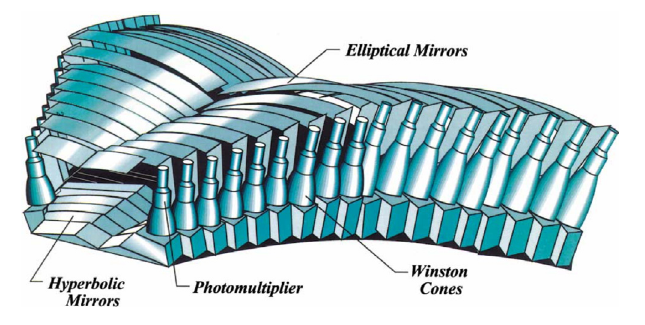
\includegraphics[width=\linewidth]{213ltcc.png}}
        \caption[LTCC Mirror System]{Layout and components of the optical mirror system within each LTCC box from the design model.}
        \label{fig::ltcc}
    \end{wrapfigure}

    The LTCC was a detector used in CLAS, which as part of the 12 GeV upgrade was refurbished to provide higher efficiency for charged pion and kaon detection.
    This was done by increasing the volume of the radiator gas, refurbishing the elliptical and hyperbolic mirrors with new coatings, and improving the sensitivity of the PMTs to Cherenkov light.
    The sensitivity improvement was achieved by coating their entrance windows with wavelength shifting material that absorbs ultraviolet (UV) light at wavelength below $300 ~\text{nm}$ and re-emits two back-to-back photons at larger wavelength \cite{ungaro2020}.
    A drawing from the design model of the LTCC can be seen in Figure \ref{fig::ltcc}.

    % !TEX root = ../main.tex
\paragraph{Forward Time-of-Flight (FTOF)}
    \begin{wrapfigure}{r}{0.50\textwidth}
        \centering\frame{
        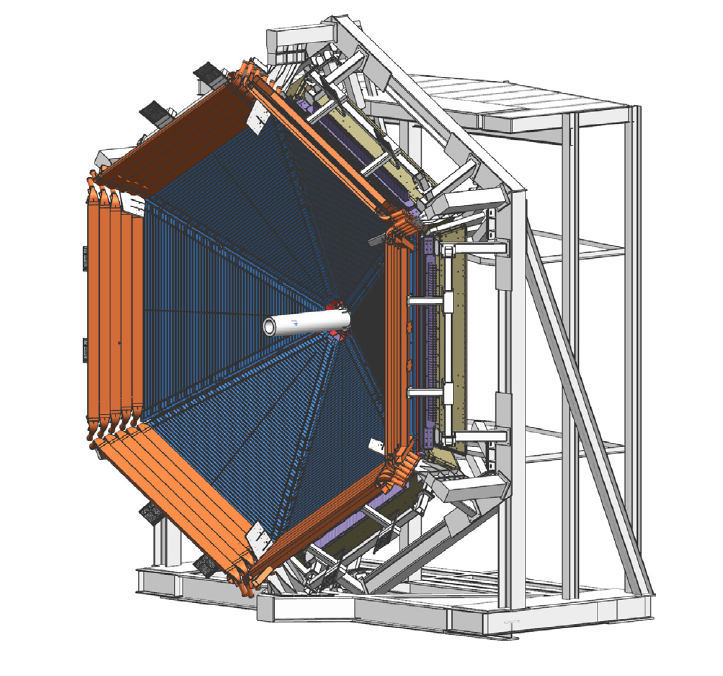
\includegraphics[width=\linewidth]{214ftof.png}}
        \caption[FTOF]{Render of the Forward Carriage with the FTOF system showing the panel-1b counters on the inside (dark blue), and the panel-2 counters on the outside (bronze).
        The panel-1a counters are located immediately downstream of the panel-1b counters and are not visible in the render.
        Part of the PCAL is visible downstream of the FTOF panels.
        Source: \hyperlink{jlab.org/physics/hall-b/clas12}{CLAS12 wiki}.}
        \label{fig::ftof}
    \end{wrapfigure}

    The FTOF system in CLAS12 is designed to measure the time-of-flight of charged particles emerging from the target during beam operation.
    It consists of six sectors of plastic scintillators with double-sided PMT readout.
    Each sector is divided into three arrays of counters separated into panels.
    Panel-1a has 23 counters, panel-1b has 62 counters, and panel-2 has 5 counters.
    The FTOF system is designed to provide excellent timing resolution for particle identification and good segmentation for flexible triggering options.
    The detectors cover a polar angle range from $5\degree$ to $45\degree$, spanning $50\%$ in azimuth at $5\degree$ and $90\%$ at $45\degree$.
    The lengths of the counters vary across the panels, ranging from $32.3 ~\text{cm}$ to $376.1 ~\text{cm}$ in panel-1a, from $17.3 ~\text{cm}$ to $407.9 ~\text{cm}$ in panel-1b, and from $371.3 ~\text{cm}$ to $426.2 ~\text{cm}$ in panel-2.

    The timing resolution achieved in the FTOF system is $125 ~\text{ps}$ in panel-1a, $85 ~\text{ps}$ in panel-1b, and $155 ~\text{ps}$ in panel-2.
    This timing resolution allows for precise measurements of the particle's time-of-flight, which is crucial for particle identification purposes \cite{carman2020ftof}.
    A render of the FTOF detector can be seen in Figure \ref{fig::ftof}.

    % !TEX root = ../main.tex
\paragraph{Ring Imaging Cherenkov Detector (RICH)}
    To improve particle identification in the momentum range of $3 - 8 ~\text{GeV}$, a RICH detector was incorporated into one of the CLAS12 sectors, replacing the corresponding LTCC sector.
    The RICH detector enhances CLAS12's capabilities in separating kaons from pions.

    The RICH detector consists of aerogel radiators, visible light photon detectors, and a focusing mirror system.
    The focusing mirror system is designed to reduce the instrumented detection area to $1 ~\text{m}^2$.
    Multi-anode PMTs are used as the photon detectors, providing the necessary spatial resolution and matching the aerogel Cherenkov light spectrum in the visible and near-UV region.

    For forward scattered particles with momenta between $3$ and $8 ~\text{GeV}$ and angles up to $13\degree$, a proximity imaging method is employed.
    This method utilises a thin ($2 ~\text{cm}$) aerogel radiator for direct Cherenkov light detection.

    For particles with larger incident angles between $13\degree$ and $25\degree$ and momenta ranging from $3$ to $6 ~\text{GeV}$, a different configuration is used.
    The Cherenkov light is produced by a thicker aerogel layer of $6 ~\text{cm}$ and focused by a spherical mirror.
    The light then undergoes two additional passes through thin radiator material and is reflected by planar mirrors before detection \cite{contalbrigo2020}.
    This setup enables efficient particle identification in this momentum and angular range.

    % !TEX root = ../main.tex
\paragraph{Electromagnetic Calorimeters (ECAL)}
\label{par::ecal}
    The CLAS12 detector package incorporates the existing electromagnetic calorimeter (EC) from the CLAS detector and adds a new pre-shower calorimeter (PCAL) upstream of the EC.
    Together, they form the ECAL, which is primarily used for the identification and kinematical reconstruction of electrons, photons, and neutrons.

    The ECAL consists of six modules, with the PCAL and EC divided into two parts each along the direction from the target.
    These parts are known as EC-inner (ECIN) and EC-outer (ECOU) and are read out separately.
    They provide longitudinal sampling of electromagnetic showers and also help improve particle identification through hadronic interactions.

    Each module has a triangular shape and is composed of 54 layers of scintillators.
    The scintillators are 1 cm thick and segmented into strips that are 4.5 cm wide for PCAL and 10 cm wide for EC, fitted between 2.2-mm-thick lead sheets.
    The total thickness of the calorimeters corresponds to approximately 20.5 radiation lengths.
    The scintillator layers are grouped into three readout views, with 5/5/8 layers per view for PCAL/ECIN/ECOU, respectively.
    This arrangement allows for spatial resolutions of less than 2 cm for energy clusters.

    To transmit the light signals from the scintillators, flexible optical fibers are used to route the light to the corresponding PMTs \cite{asryan2020}.

    % !TEX root = ../main.tex
\paragraph{Forward Tagger (FT)}
    The FT is an extension of the CLAS12 detector that allows for the detection of electrons and photons at very forward polar angles, specifically ranging from $2.5\degree$ to $4.5\degree$.
    By detecting forward-scattered electrons, the FT enables electroproduction experiments at low photon virtuality $Q^2$, providing a high-intensity, linearly polarized, quasi-real photon beam with energy tagging.
    This setup is particularly suitable for hadron spectroscopy studies.

    The FT consists of three main components: the FTCal (calorimeter), the FTTrk (micro-strip gas tracker), and the FTHodo (hodoscope).
    The FTCal utilises 332 lead-tungstate ($\text{PbWO}_4$) crystals to identify electrons, measure the energy of electromagnetic showers, and provide fast trigger signals.
    The FTTrk, located in front of the FTCal, is responsible for measuring the scattering angles of charged particles.
    The FTHodo, a scintillator detector, assists in the separation of electrons and high-energy photons.

        \begin{wrapfigure}{l}{0.50\textwidth}
            \centering\frame{
            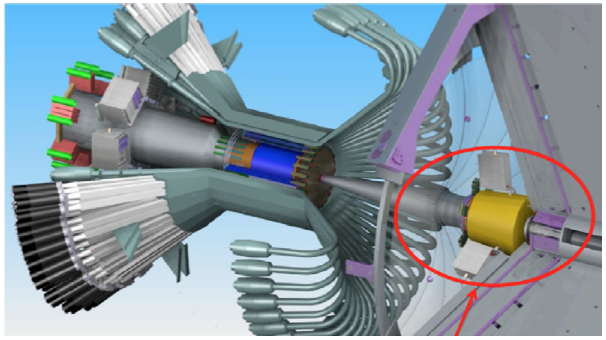
\includegraphics[width=\linewidth]{217ft.png}}
            \caption[FT]{The Forward Tagger system circled downstream of the CD in front of the torus magnet warm bore entrance.
            Source: \hyperlink{jlab.org/physics/hall-b/clas12}{CLAS12 wiki}.}
            \label{fig::11.217::ft}
        \end{wrapfigure}

    During beam operations, a conical tungsten shielding pipe is placed in front of the FT to absorb M\o ller electrons and low-energy photons generated by beam interactions with the target and downstream materials.
    This shielding not only protects the FT and Forward Detectors from electromagnetic background but also ensures compatibility with the FT acceptance.
    This configuration, referred to as ``FT-ON'', allows the FT to detect both electrons and photons, expanding the detection capabilities of CLAS12.

    Alternatively, when the FT is not required for the specific physics program, the FT detectors can be turned off, and additional shielding elements are installed in front of the FT, covering up to $4.5\degree$ of polar angle.
    This modified configuration, known as "FT-Off," reduces accidental background by one-third under the same beam conditions, enabling higher luminosity data acquisition with CLAS12 by mitigating background interference from the DC R1 chambers \cite{acker2020ft}.

